\documentclass[tikz]{standalone}

\begin{document}
\definecolor{printred}{RGB}{215,25,28}
\definecolor{printorange}{RGB}{253,174,97}
\definecolor{printyellow}{RGB}{255,255,191}
\definecolor{printgreen}{RGB}{145,180,130}
\definecolor{printblue}{RGB}{43,131,186}
\definecolor{printlilac}{RGB}{178,171,210}
  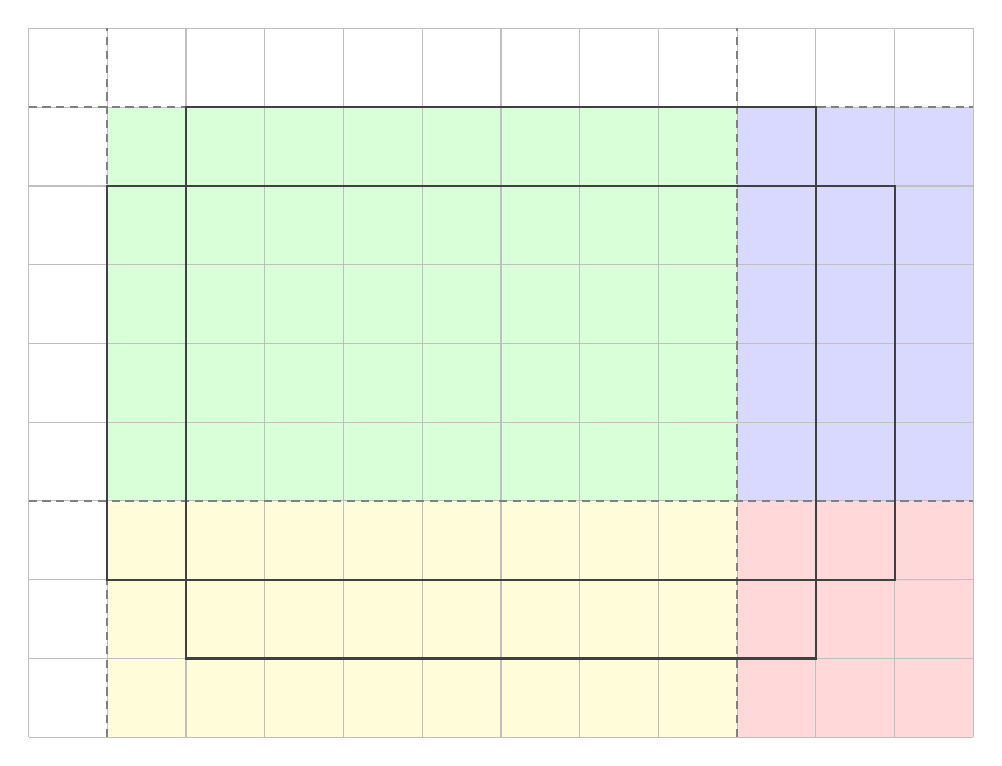
\begin{tikzpicture}[scale=1.0]

    % Drawing Parameters
    \pgfmathsetmacro{\leftgap}{1}%
    \pgfmathsetmacro{\topgap}{1}%
    \pgfmathsetmacro{\rightgap}{3}%
    \pgfmathsetmacro{\bottomgap}{3}%
    \pgfmathsetmacro{\innerwidth}{8}%
    \pgfmathsetmacro{\innerheight}{5}%


    % Intermezzo values
    \pgfmathsetmacro{\figureheight}{\topgap+\innerheight+\bottomgap}%
    \pgfmathsetmacro{\figurewidth}{\leftgap+\innerwidth+\rightgap}%

    %% Here Be Dragons!
    %Pastel boxes
    % TODO - prefer text; p(i, j); p(i+1, j); p(i, j+1); p(i+1, j+1)
    \fill[green!15!white] (\leftgap, \bottomgap) rectangle (\leftgap+\innerwidth, \bottomgap+\innerheight);
    \fill[blue!15!white] (\leftgap+\innerwidth, \bottomgap) rectangle (\figurewidth, \bottomgap+\innerheight);
    \fill[red!15!white] (\leftgap+\innerwidth, \bottomgap) rectangle (\figurewidth, 0);
    \fill[yellow!15!white] (\leftgap, 0) rectangle (\leftgap+\innerwidth,\bottomgap);

    \draw[lightgray, thin, step=1] (0,0) grid (\figurewidth,\figureheight);
    % Vertical Dashes
    \draw[gray, semithick, densely dashed] (\leftgap,0) -- (\leftgap, \figureheight);
    \draw[gray, semithick, densely dashed] (\leftgap+\innerwidth,0) -- (\leftgap+\innerwidth, \figureheight);

    % Horizontal Dashes
    \draw[gray, semithick, densely dashed] (0,\bottomgap) -- (\figurewidth,\bottomgap);
    \draw[gray, semithick, densely dashed] (0,\bottomgap+\innerheight) -- (\figurewidth,\bottomgap+\innerheight);

    % T+1 A.O.R
    % Centre
    \draw[darkgray, thick] (\leftgap+1,\bottomgap-1) rectangle (\leftgap+\innerwidth+1, \bottomgap+\innerheight-1);
    % North Boundary
    \draw[darkgray, thick] (\leftgap+1,\bottomgap+\innerheight) rectangle (\leftgap+\innerwidth+1, \bottomgap-2);
    % South Boundary
    \draw[darkgray, thick] (\leftgap+1,\bottomgap-1) rectangle (\leftgap+\innerwidth+1, \bottomgap-2);
    % East Boundary
    \draw[darkgray, thick] (\leftgap+\innerwidth+1,\bottomgap-1) rectangle (\leftgap+\innerwidth+2, \bottomgap+\innerheight-1);
    % West Boundary
    \draw[darkgray, thick] (\leftgap,\bottomgap-1) rectangle (\leftgap+1, \bottomgap+\innerheight-1);
  \end{tikzpicture}
\end{document}
